\documentclass[a4paper, 11pt]{article}
\usepackage[mode=buildnew]{standalone}
\usepackage[utf8]{inputenc}
\usepackage[margin=2.5cm]{geometry}
\usepackage{graphicx}
\usepackage{siunitx}
\usepackage{float}
\usepackage{microtype}
\usepackage{subcaption}
\usepackage{caption}
\captionsetup{font=small}
\captionsetup[subfigure]{width=0.9\linewidth}
\captionsetup[figure]{width=0.8\linewidth}
\captionsetup[table]{width=0.8\linewidth}
\usepackage{hyperref}
\usepackage{amsmath}
\usepackage[nameinlink,noabbrev,capitalise]{cleveref}
\usepackage{booktabs}
\usepackage{tabulary}
\usepackage{appendix}
\usepackage{tikz}

\usepackage{import}

\usepackage{fancyhdr}
\setlength{\headheight}{14pt}
\fancyhead[L]{Integrated Design Project}
\fancyhead[R]{}
\pagestyle{fancy}

\title{IDP Report}
\author{L221}
\date{February 2021}


\usepackage{titling}
\makeatletter
\renewcommand{\maketitle}{
\begin{titlingpage}
\begin{center}
    \vspace*{4cm}
    {\Huge\bfseries\@title}\par
    \vspace*{2cm}
    \Large
    \@author\par\bigskip
    Trinity College\par
    \vspace*{2cm}
    \@date
\end{center}
\end{titlingpage}
}
\makeatother


%%--------------------------------------------------------------------------
%% Code Highlighting
%%--------------------------------------------------------------------------

\usepackage{xcolor}
\usepackage{listings}
\definecolor{pyorange}{RGB}{255,119,0}
\definecolor{pyblue}{RGB}{0,0,255}
\definecolor{pypurple}{RGB}{144,0,144}
\definecolor{pyred}{RGB}{221,0,0}
\definecolor{pygreen}{RGB}{0,170,0}
\definecolor{pyblack}{RGB}{0,0,0}
\lstdefinestyle{pystyle}{
    commentstyle = \color{pygreen},
    keywordstyle = \color{pyblue},
    stringstyle = \color{pyorange},
    basicstyle = \small\color{pyblack}\ttfamily,
    breaklines = true, %automatic line breaking of long lines      
    numbers = left,
    numberstyle=\tiny,
    showstringspaces = false,
    stepnumber = 2,
	xleftmargin=17pt,
	captionpos=b
}
\lstset{style=pystyle,language=Python}


%%--------------------------------------------------------------------------
%% References
%%--------------------------------------------------------------------------

\usepackage[style=nature]{biblatex}
% \bibliography{bibliography.bib}


% - Mechanical
% - Sketches of the concepts you have considered (which may be photocopied/scanned from your lab book). Evaluation charts of these concepts together with a brief discussion of the advantages and disadvantages of each
% - *Robot Concept and diagram.* This could be hand-drawn diagrams, CAD models or any format which conveys the approach and concept

% - Electrical
% - *Electronics/Sensing.* This should include a list of sensors/circuits required, any circuit diagrams/block diagrams which may have already been developed. Discussion as to if/why some processing will be performed in electronics opposed to software (e.g. obtaining digital outputs from analogue signals)
% - Overall System Level Diagram. Detailing how the electronics, hardware and software interacts
% - Integration between hardware electronics and software

% - What is the most risky/challenging aspect of the project?
% - Gantt Chart (resource/time allocation)
% - Approach for solving the problem

% - Software
% - *Software.* Exploration and navigation algorithms. Interface to electronics, discussion of choice of algorithms, any failure detection/recovery which will be implemented.



\begin{document}

\maketitle

\section{Introduction}
\subsection{Project Management}
\subsection{Team organisation}

The team is divided into 3 sub-teams, each holding responsibility for the progress of one aspect of the project; we have a mechanical, electrical and software sub-team. The team is split with Youjing and Care (Raksina) in the mechanical team, Eleanor and Karl in the electrical team and Weixuan, Jason and Ghifari in the software team. We also have Ghifari as the team leader, responsible for project management.


Although we have these 3 distinct teams, an interdisciplinary approach is taken. All 3 teams are in constant communication to ensure that a holistic view is taken for any decisions made. This is true for anything from the Overall Robot Strategy to the chassis design.

\subsection{Approach}

Our approach to tackling this problem is to use the Agile methodology. First, we collectively agreed on a Minimum Viable Product (MVP) that we aim to create as soon as possible. Once this is created, we go through week long iterations of optimising and overcoming any problems before a review every Saturday. In this way we have a clear direction in terms of what we need to achieve with a clear deadline.

The current MVP comprises of a few details from each team. From the mechanical team, it is a simple model of the chassis in Webots with rough dimensions, from the electrical team, it is to create the lookup tables for the sensors we will be using (long IR and ultrasonic sensors) and from the software team, it is a robot with simple motion controls that can detect a block and go towards it.

\subsection{Gantt Chart}

\begin{figure}[H]
    \centering
    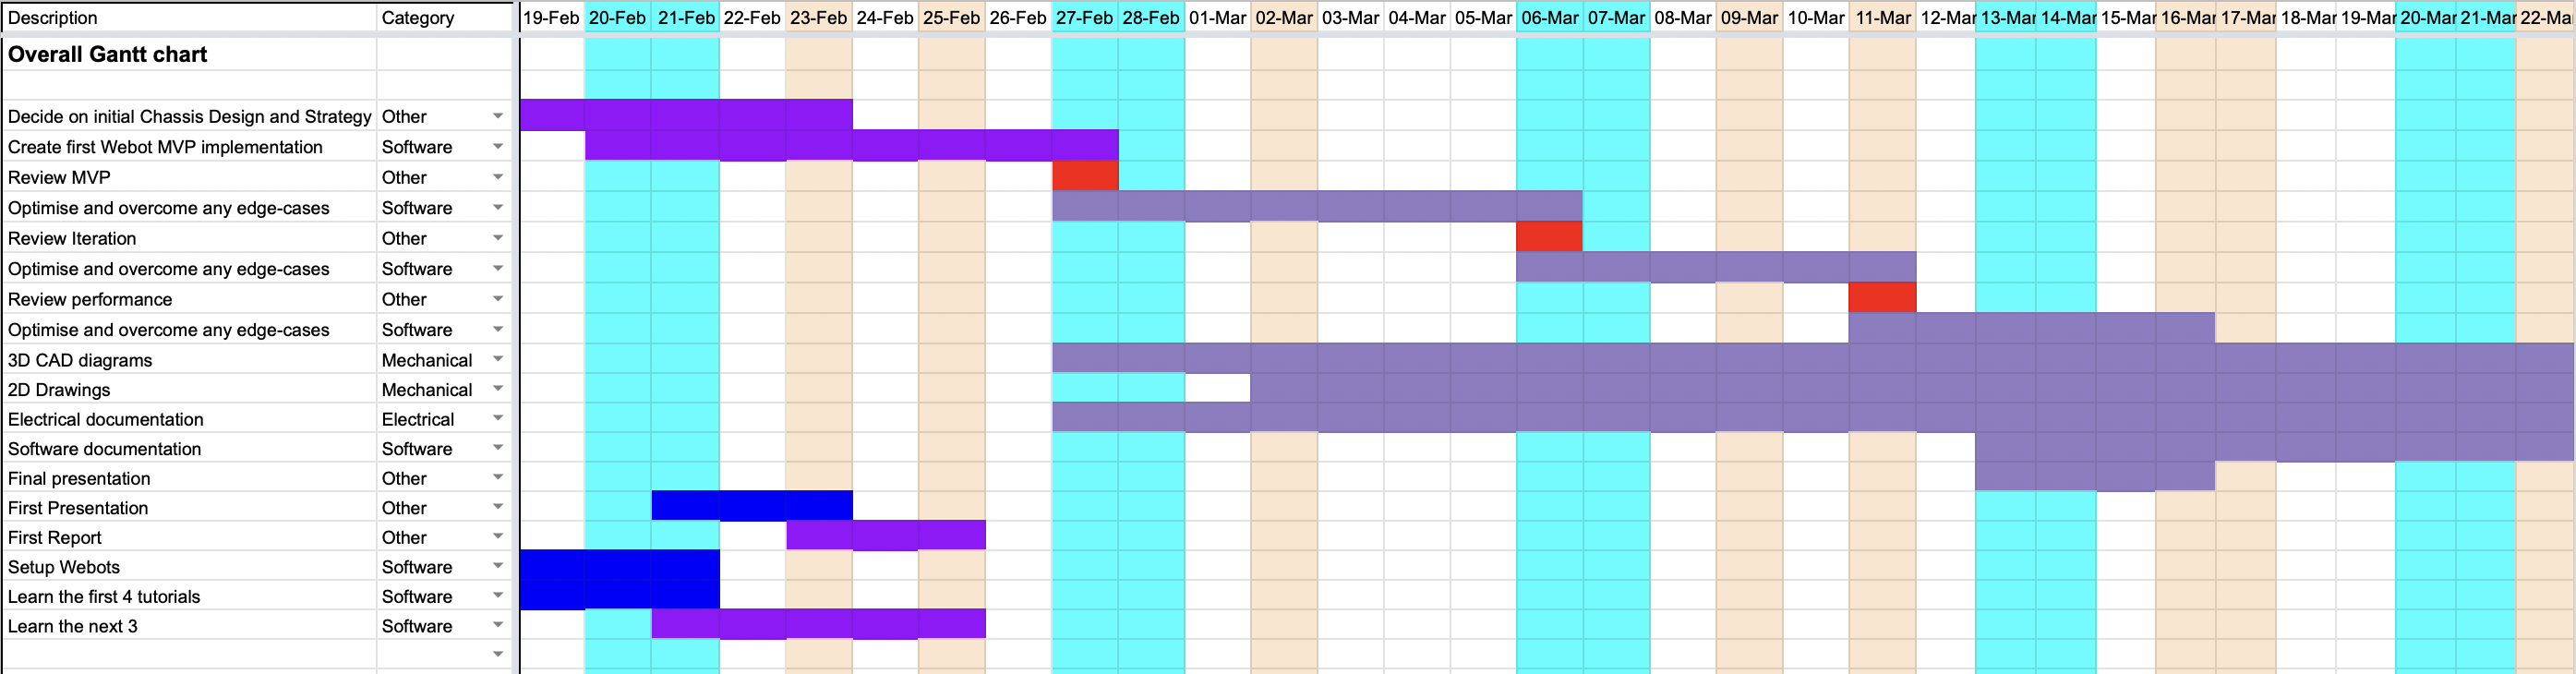
\includegraphics[width=14cm]{GanttChart}
    \caption{Overall team Gantt Chart}
\end{figure}

Figure 1 shows our Gantt Chart for the project. We are currently in progress to meet the MVP deadline of this Saturday, which is currently the most critical path. Saturday's meeting will enable important tasks to start such as the 3D CAD drawings and electrical documentation.
\section{Mechanical}
\subsection{Initial Designs}

\begin{figure}[H]
    \centering
    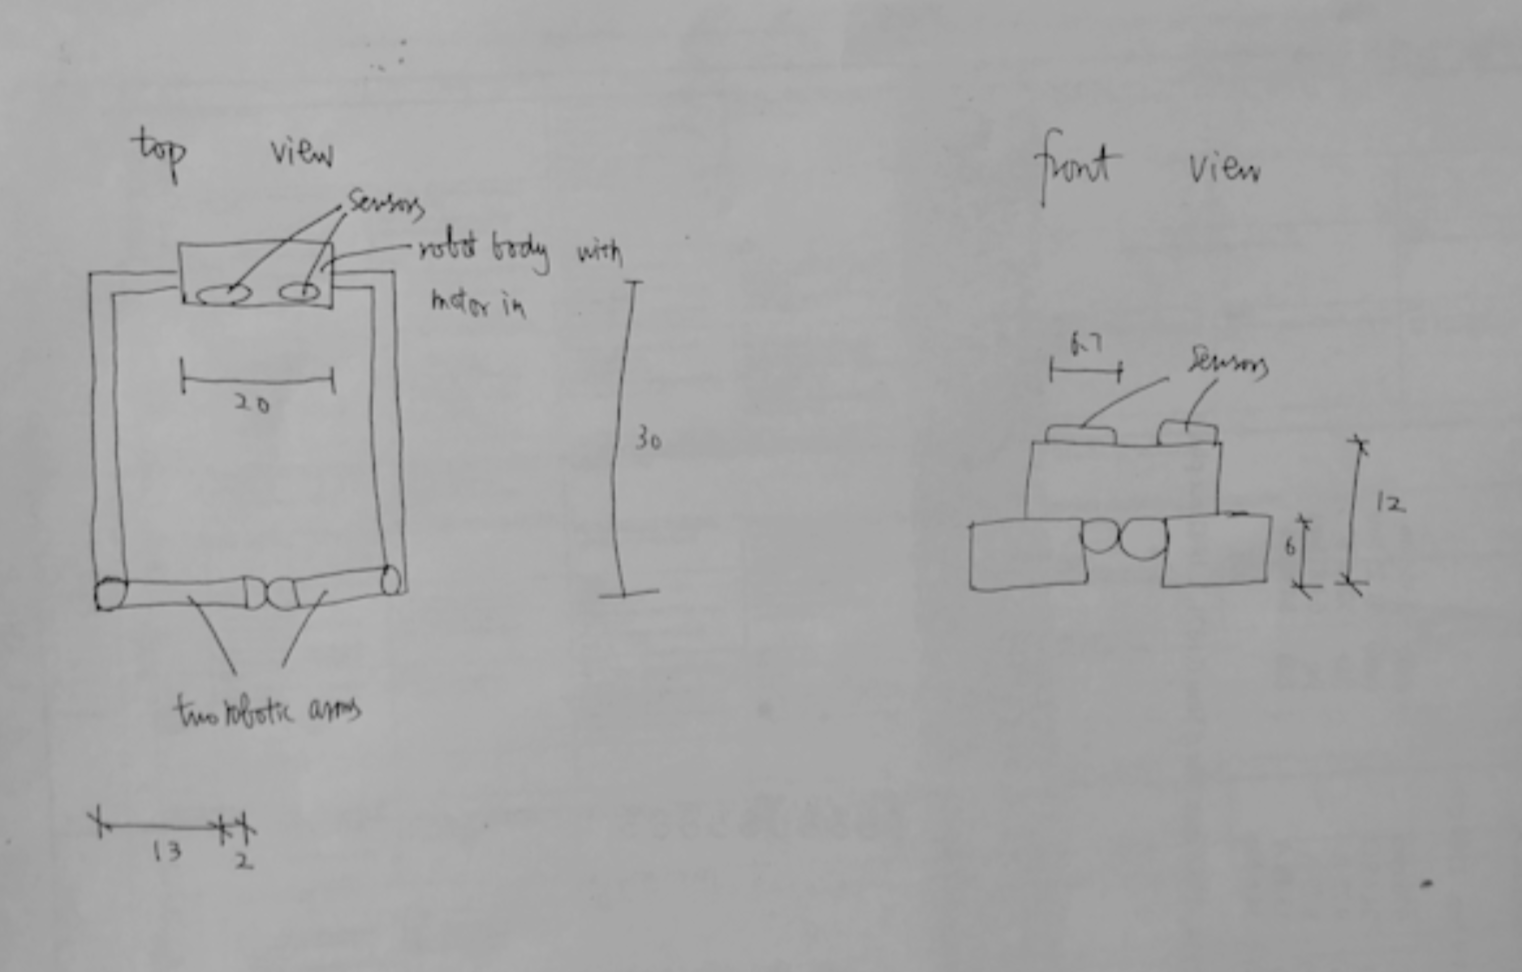
\includegraphics[width=8cm]{Design1}
    \caption{The First Design}
    \label{}
\end{figure}


The pros of the designs are that it is symmetric so it will be easier for sensor construction and placement. It is also considered relatively simple. However, this design suffers from the shortcomings that the sensor is at the back of the robot, which makes it difficult for the blocks to be accurately detected. The square shape also makes it difficult to rotate. 


\begin{figure}[H]
    \centering
    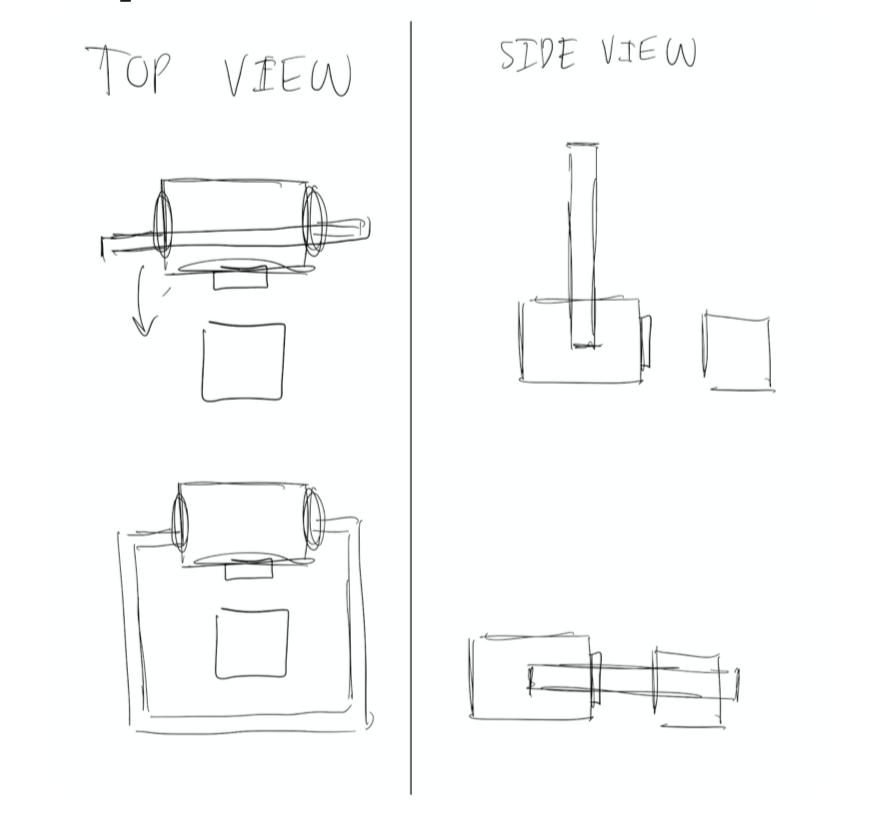
\includegraphics[width=8cm]{Design2}
    \caption{The Second Design}
    \label{}
\end{figure}


Based on the advantages and disadvantages of the first design we have come up with the second design. Instead of the arms rotating in the plane of the floor but up and down now. The advantage is that this design is still simple and symmetric. However, it suffers from the main fault that the sensor becomes useless once a block is collected. So it is not suitable for gathering multiple blocks.

\subsection{Preferred Design}


\begin{figure}[H]
    \centering
    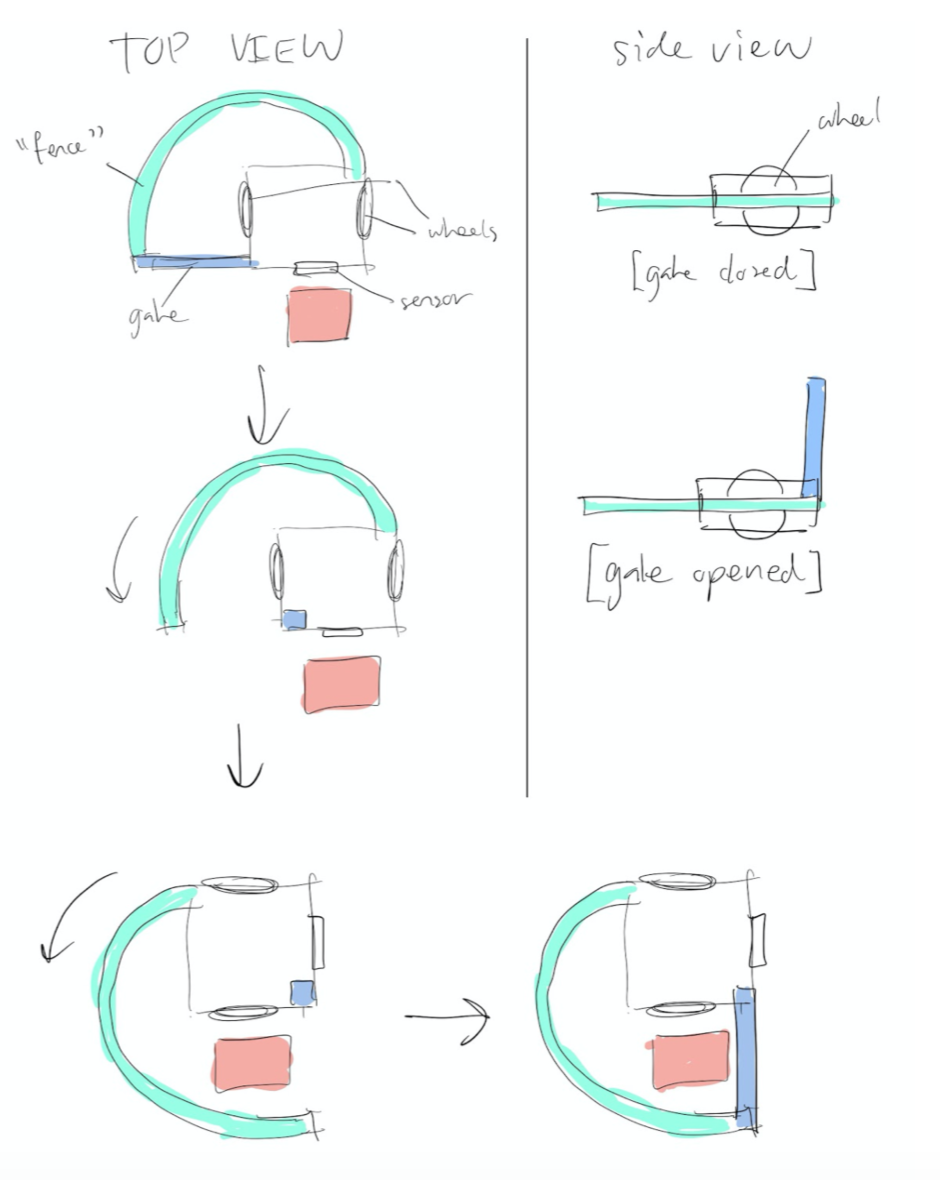
\includegraphics[width=8cm]{Design3}
    \caption{The Preferred Design}
    \label{}
\end{figure}


Here is our preferred design, which has a semi-circular arm that keeps the blocks in on the way of collecting the blocks. This design is simple, suitable for collecting multiple blocks and it is easy to allocate sensors on the robot body. The circular shape also makes it easier to rotate. However, its asymmetric nature still makes the robot prone to sway to one side. It also needed to rotate to collect to collect blocks which may increase complexity.









\section{Electrical}

\subsection{Sensor choices}

% IR Modelling graphs

% Something about .proto files

% Color sensing

\subsection{Initial electronics list}

% Arduino

% Motor shield

% Sensors

% Battery pack

% Any other useful discrete electronics


\section{Strategy and Software}



\subsection{Overall Strategy and Electrical Integration}
\label{sec:software_flow_chart}

The main controller can be divided into four parts, the overall software flow chart is shown in \cref{fig:flow_overall}. The four parts are exploration and target selection algorithm, navigation and motion control, block collect control, emergency interrupts. 

We employed a coordinate system based approach, with heavy use of the GPS and compass data. This approach, at a higher level, will allow more complicated strategies, as well as preventing collisions with the other robot and walls without any sensors. However, sensors are still used for interrupts, in additional to exploration and target selection.











\newpage
\begin{figure}[H]
    \centering
    \includestandalone[width=0.8\textwidth]{./flowchart/overall}
    \caption{The overall software flowchart}
    \label{fig:flow_overall}
\end{figure}
\newpage



\subsection{Exploration and Target Selection}\label{subsec:target}

to determine the target, a greedy algorithm, where the closest block is chosen as the target, will be used (see \cref{subsec:target}).

\begin{figure}[H]
    \centering
    \includestandalone[width=0.3\textwidth]{./flowchart/target_detect}
    \caption{The exploration algorithm}
    \label{fig:flow_target}
\end{figure}




\subsection{Navigation and Motion Control}

The robot moves according to a queue of target actions, involving target coordinates and rotations.

% this only works locally big rip
\begin{figure}[H]
    \centering
    \includestandalone[width=0.5\textwidth]{./flowchart/control_flow}
    \caption{Control logic for getting to a target}
    \label{fig:flow_motion}
\end{figure}

% I've included pretty much all the detail here so feel free to delete anything if needed, just make sure you understand first so you know what's deleted.

The motion control works by calculating wheel velocities based on the distance and the clockwise angle from the robot to target as illustrated in figure \ref{fig:flow_motion}. 3 parameterised methods are available for making this calculation. Each calculates a forward and rotational velocity, $V_f$ and $V_r$ respectively, which are combined to give velocities for each wheel motor. The left motor velocity is $V_f + V_r$ and the right motor is $V_f - V_r$. If the angle is negative the signs on $V_r$ are reversed. These outputs represent the fraction of the motors total drive. If any drive ends up over 1 it's capped at that value. For different actions i.e. rotate, drive to point etc. different methods can be used with different parameters. 

The first method is purely angle based and is currently used for driving to positions. The velocities are given by the following equations where a and b are free parameters and x is the inputted angle. Currently a=3 and b=0.5.

\begin{equation}
    V_f = 
    \begin{cases} 
      0 & x\leq \frac{-\pi}{2} \\
      cos^a(x) & \frac{-\pi}{2} \leq x\leq \frac{\pi}{2} \\
      0 & \frac{\pi}{2} \leq x 
   \end{cases}
\end{equation}

\begin{equation}
    V_r = (\frac{|x|}{\pi})^b
\end{equation}

The second method uses proportional control based on distance error for $V_f$ and angle error for $V_r$. Once combined into left and right velocities the result is passed through a sigmoid scaled to be from -1 to 1. In future this method will use full PID control. This method is currently used to face the robot at a particular bearing.

The third method uses a short linear region. In the equations below, a through d are parameters for the method and x and y are the distance and angle errors respectively. This method is used for rotating at constant rates with b and d being small.

\begin{equation}
    V_f = 
    \begin{cases} 
      -a & x\leq -b \\
      \frac{ax}{b} & -b \leq x\leq b \\
      a & b \leq x 
   \end{cases}
\end{equation}

\begin{equation}
    V_r = 
    \begin{cases} 
      -c & y \leq -d \\
      \frac{cy}{d} & -d \leq y \leq d \\
      c & b \leq y 
   \end{cases}
\end{equation}

% \subsection{Other Subsystems}

% \begin{figure}[H]
%     \centering
%     \includestandalone[width=0.3\textwidth]{./flowchart/collect}
%     \caption{todo}
%     \label{fig:flow_collect}
% \end{figure}



\subsection{Evaluation and Improvements}

% Other btec algo

Other algorithms and strategies were considered, for example, spiralling outwards from the starting point and collect blocks along the path. However, we think that the current strategy is more efficient, and have a higher potential while with similar feasibility. One of the main challenges of the spiral approach is keeping both robots on their spiral track without collisions, while keeping the strategy symmetric between the two robots running the same piece of control software.


% Potential failure

A properly programmed target selection algorithm should limit the number of potential collisions, since the target coordinate will be checked against walls or the other robot when it is picked. However, this does not guarantee that the paths of motion of the two robots will not intersect after they start moving, so an emergency interrupt is crucial.

There is an extremely low probability that after the collision interrupt, the target choosing algorithm will pick the same target that triggered the interrupt, and the interrupt will be triggered again. In principle, this should not result in an infinite loop, since the main cause of an interrupt is the other robot, which should have moved after a few iterations.

In an unlikely situation, the distance sensors will not detect anything in the initial target selection phase. However, since the target selection algorithm will greedily choose the closest detected coordinate, which is guaranteed to exist (even if it is not an actual block but noise from the sensor), the algorithm will not stall.





A potential difficulty arises when the target block is of the wrong colour, which the target selection algorithm has to ignore. This can be partially solved by keeping a list of failed target coordinates as blacklisted regions, however, the block collector design would require the robot to drive backwards to preventing hitting the wrong block away from its current location.





% Improvements

Potential improvements to the current strategy after the MVP includes communication of coordinates of detected blocks of the wrong colour between robots, which will be inserted to the target priority queue with a higher profit. Furthermore, advanced probabilistic path planning can be implemented. 


% Not sure where to put this

\subsection{Future Problems and Risks}

While planning this project, we thought about where there may be difficulties in the future. We have listed these problems will try to find solutions to them when our robot has progressed.

Firstly, the position of the are may cause trouble. Since the two areas are in the middle of the arena, this may disrupt the pathing of the robots if collected blocks are in the arena. Our current solution is to create a robot that will collect all the blocks at once, thus preventing this problem to occur at all.

Picking up the blocks may also be troublesome. Once the robot has detected and moved towards the block, it then needs to position itself correctly in order to pick up the block. How accurate this needs to be will need to be seen once we start testing our robot.

Another potential problem is ensuring there are no problems. The robot will need to constantly be processing information to ensure that it will not collide with anything. Since there are 2 robots, this may prove tricky to coordinate and a fall back mechanism will need to be developed.

\end{document}
